\documentclass[runningheads]{llncs}
%
\usepackage[T1]{fontenc}
% T1 fonts will be used to generate the final print and online PDFs,
% so please use T1 fonts in your manuscript whenever possible.
% Other font encondings may result in incorrect characters.
%
\usepackage{graphicx}
% Used for displaying a sample figure. If possible, figure files should
% be included in EPS format.
%
\usepackage{amsmath}
\usepackage{amssymb}
\usepackage{mathtools}
\usepackage{float}
\usepackage[utf8]{inputenc}
\usepackage{tikz}
\usetikzlibrary{shapes.geometric, arrows, positioning, calc, backgrounds, fit} % Librerías de TikZ

% --- Configuración de Estilos ---
\tikzstyle{startstop} = [rectangle, rounded corners, minimum width=3cm, minimum height=1cm,text centered, draw=black, fill=gray!10, font=\small\bfseries]
\tikzstyle{process} = [rectangle, minimum width=3.5cm, minimum height=1cm, text centered, draw=black, fill=white, font=\small]
\tikzstyle{decision} = [diamond, aspect=2, minimum width=3cm, minimum height=1cm, text centered, draw=black, fill=white, font=\small]
\tikzstyle{arrow} = [thick,->,>=stealth]
\tikzstyle{container} = [draw, rectangle, dashed, inner sep=0.5cm, rounded corners]

% If you use the hyperref package, please uncomment the following two lines
% to display URLs in blue roman font according to Springer's eBook style:
%\usepackage{color}
%\renewcommand\UrlFont{\color{blue}\rmfamily}
%
\begin{document}
%
\title{Trajectory Planning for a 2-DOF Manipulator Robot to Minimize Overall Energy Consumption\thanks{Supported by Universidad de Guadalajara}}
%
\author{Jonathan Piña-Orlaineta \and Michel Lopez-Franco \and Jesus Hernandez-Barragan \and Carlos Lopez-Franco}
%
% First names are abbreviated in the running head.
% If there are more than two authors, 'et al.' is used.
%
\institute{Centro Universitario de Ciencias Exactas e Ingeniería, Guadalajara Jalisco 44430, México \\
\email{jonathan.pina7309@alumnos.udg.mx}}
%
\maketitle

\begin{abstract}
This paper presents an energy-efficient trajectory planning approach for a 2-DOF manipulator robot based on cubic spline interpolation and Particle Swarm Optimization (PSO). Smooth joint trajectories are computed using cubic splines, while PSO determines optimal intermediate joint configurations that minimize energy consumption. The optimization is guided by a cost function defined as the integral of squared joint torques, including penalty terms on maximum torque and joint velocity to ensure dynamically feasible and safe operation. Simulation results show that the optimized trajectory redistributes dynamic effort throughout the motion, producing smoother torque and bounded velocity profiles compared to an arbitrary trajectory. The proposed method achieved a 26.86\% reduction in total energy consumption while slightly decreasing peak torque values, demonstrating improved energetic efficiency without modifying execution time or robot hardware. 

Although performance depends on parameter tuning and accurate modeling, the results highlight the potential of combining spline-based trajectory generation with evolutionary optimization for energy-aware robotic motion planning.

\keywords{Energy saving  \and Manipulator robot \and Trajectory planning \and Evolutionary computation \and {Polynomial interpolation}.}
\end{abstract}
%
%
%
\section{Introduction}
The consolidation of Industry 4.0 and the transition to Industry 5.0~\cite{ref_industry5.0,ref_ind5.0_capabilities} is driving a massive demand for programmable electromechanical systems, highlighting industrial robots (IRs) as pillars of global efficiency and productivity. As reported by the International Federation of Robotics in its most recent document Executive Summary World Robotics 2025 Industrial Robots, approximately 542,000 units were installed worldwide, reaching a historical operating stock of more than 4.6 million robots. This remarkable growth is led by the Asia and Australia regions, which report the highest number of installations of these systems, with just over 400,000 units~\cite{ref_wr2025}.

This trend inevitably results in an increase in global energy consumption. In 2023, the International Energy Agency reported that the industrial sector is the main consumer of electricity worldwide, with 42\% of all final electricity consumed by the main sectors, including transport, residential, commercial and utilities, agriculture, fishing and other unspecified sectors~\cite{ref_iea}. Specifically, countries or regions that are pioneers in the installation and use of these systems as part of their production chain, such as the United States and China, have reported upward trends in terms of electricity consumption in this sector in recent years. In the case of the United States, the U.S. Energy Information Administration reported an annual increase in electricity consumption of 2.1\% from 2020 to date~\cite{ref_eia}; while, in China, CEIC Data reports that, from 2012 to 2022, the increase in electricity consumption in the industrial sector has been 58\%~\cite{ref_ceic}.

Several works have addressed the problem of energy consumption in robotic systems through trajectory optimization. Soori et al.~\cite{soori2023} provide a comprehensive review of energy-saving strategies for industrial robots, identifying trajectory planning as one of the most effective approaches for reducing energy expenditure without hardware modifications. Building on this premise, metaheuristic methods have been 
widely explored: Zhou et al.~\cite{zhou2024} combine an improved sparrow search algorithm with B-spline interpolation to minimize energy in welding robots, while Zhang et al.~\cite{zhang2023} formulate a multi-objective deep reinforcement learning approach for six-axis manipulators, 
simultaneously optimizing energy consumption, tracking accuracy, and motion smoothness. In the context of planar manipulators, Garriz and Domingo~\cite{garriz2022} optimize trajectories for a 6-DOF industrial robot by simultaneously maximizing manipulability and minimizing electrical energy via the Kalman method.

In this paper, a novel, simpler, yet effective methodology for minimizing energy consumption of a 2-DOF RR manipulator robot through the integration of Particle Swarm Optimization (PSO) and the generation of smoothed trajectories with high-degree polynomials is proposed. The main contribution lies in the formulation of a multi-objective cost function incorporating torque penalty terms, which acts as a dynamic regulator that not only optimizes electrical efficiency, but smooths out torque profiles, ensuring that actuators operate within safe ranges to extend their service life and reduce the need for corrective maintenance.

\section{Background}
This section presents the theoretical foundations and mathematical formulations that support the development of the present work. First, the dynamic modeling of a robotic manipulator is introduced, along with the most commonly used energy computation metrics in the context of energy optimization in robotic systems. Subsequently, the concept of polynomial interpolation and its application to trajectory planning in robotics are described, highlighting its relevance in generating smooth and dynamically feasible motion profiles. Finally, the PSO algorithm is presented, emphasizing its fundamental principles and the advantages it offers when addressing nonlinear optimization problems with multiple constraints.

\subsection{Robot dynamics model}
 The system used for this work was a 2-DOF manipulator robot with revolute joints. Figure \ref{fig:man_robot} shows a sketch of this system. Both revolute joints are actuated by their respective engines, each generating a complete DOF. It is observed that $l_1$ and $l_2$ are the fixed lengths of the manipulator’s links, $r_1$ and $r_2$ are the distances towards the center of mass of each link measured with respect to their respective joint axes, $\theta_1$ and $\theta_2$ are the joint variables of the manipulator. The global coordinate frame $x-y$ is located on the revolute joint axis that controls link 1.

\begin{figure}[H]
    \centering
    
\includegraphics[width=0.5\textwidth]{figures/man_robot_sketch.png}
    \caption{Sketch of a 2-DOF manipulator robot.}
    \label{fig:man_robot}
\end{figure}

The basis of any effort to optimize the energy consumption of a robot lies in the accuracy of its dynamic model. For $n$-DOF manipulators, the technical literature mostly uses the Euler-Lagrange formulation, which describes the relationship between the applied forces/torques and the resulting movement of the links. The differential equation governing this behavior~\cite{ref_dynamics1,ref_dynamics2} is expressed as follows:

\begin{equation}
    \boldsymbol \tau = \textbf{M}(\boldsymbol \theta) \boldsymbol {\ddot \theta} + \textbf{c} (\boldsymbol \theta, \boldsymbol{\dot \theta})+ \textbf{g}(\boldsymbol \theta)
\end{equation}

where $\boldsymbol \theta \in \mathbb{R}^n$ is the angular position vector (in this case, $\boldsymbol \theta=[\theta_1,\theta_2 ]^T$), $\textbf{M}(\boldsymbol \theta)\in \mathbb{R}^{n\times n}$  is the inertia matrix, $\textbf{c}(\boldsymbol \theta , \boldsymbol{\dot \theta})\in \mathbb{R}^n$ contains the effects of Coriolis and centrifugal on the system, $\textbf{g}(\boldsymbol \theta)\in \mathbb{R}^n$ is the vector of gravity torques. For the sake of brevity, the shorthand trigonometric notation $c_j \coloneqq \cos(\theta_j)$, $s_j \coloneqq \sin(\theta_j)$ (for $j\in \{1, 2\}$), and  $c_{12} \coloneqq \cos(\theta_1 + \theta_2)$ is adopted throughout this section.

For a 2-DOF manipulator robot, the inertia matrix $\textbf{M}(\boldsymbol \theta)$ has the following form:

\begin{equation}
    \textbf{M}(\boldsymbol \theta)=\begin{bmatrix} I_1+I_2+m_1r_1+m_2(l_1^2+r_2^2+2l_1r_2c_2) & I_2+m_2(r_2^2+l_1r_2c_2) \\ I_2+m_2(r_2^2+l_1r_2c_2) & I_2+m_2r_2^2\end{bmatrix}
\end{equation}
where $I_1$ y $I_2$ are inertia of links 1 y 2, respectively, while $m_1$ y $m_2$ are their masses. Note that $[\textbf{M}]_{21}=[\textbf{M}]_{12}$.

The Coriolis vector $\textbf{c}(\boldsymbol \theta,\boldsymbol{\dot \theta})$ for the same system is defined as follows:

\begin{equation}
    \textbf{c}(\boldsymbol \theta, \boldsymbol{\dot \theta}) = \begin{bmatrix} -m_2l_1r_2s_2(2\dot \theta_1\dot \theta_2+\dot \theta_2^2) \\ m_2l_1r_2 \dot \theta_1 ^2s_2
    \end{bmatrix}
\end{equation}

Finally, the gravity vector $\textbf{g}(\boldsymbol \theta)$ is defined as follows:

\begin{equation}
    \textbf{g}(\boldsymbol \theta)=\begin{bmatrix}
        (m_1r_1+m_2l_1)g c_1 + r_2g c_{12} \\ m_2r_2g c_{12}
    \end{bmatrix}
\end{equation}

where $g$ is the Earth's gravitational acceleration constant.

\subsection{Energy consumption metrics}
The consumption of electrical energy in actuators is not limited only to the mechanical work carried out by the robot. Electric motors dissipate energy through losses in copper and losses in iron, in addition to the consumption of the brake and control systems. Therefore, the energy cost index $E$ used in optimization is usually computed in two main forms: using the instantaneous power integral, which is calculated by the inner product between the torque and angular velocity vectors, or the integral of the L2 torque norm, the latter being a common approach to minimize heating of motors and associated electrical consumption~\cite{ref_dynamics2}. Both metrics are represented as follows, but only the square torque metric (equation \ref{tau2_metric}) was used:

\begin{equation}
    E=\int_0^T |\boldsymbol \tau (t) \cdot \boldsymbol{\dot \theta} (t)| dt
\end{equation}

\begin{equation}\label{tau2_metric}
    E=\int_0^T \sum_{i=1}^n \tau_i^2 (t) dt
\end{equation}

In both metrics, $T$ is the desired operation time for the robot in seconds.
The complexity of these models increases with the number of links and the presence of dynamic couplings, which makes the search for the optimal path a non-linear, non-convex and highly constrained optimization problem.

\subsection{High-degree polynomial interpolation}
Polynomial interpolation is defined as the mathematical technique of constructing a continuous function, specifically a polynomial of the form $P(t) = a_n t^n + a_{n-1} t^{n-1} + \dots + a_1 t + a_0$, that passes exactly through a given set of points or \textit{waypoints}. In the context of robotics, these points typically represent joint angles in joint space or positions and orientations in the operational space. The main objective of trajectory generation is to provide the motion control system with a continuous stream of setpoints—including position, velocity, and acceleration—that will serve as a guide to move the robot under the desired kinematic constraints~\cite{ref_polyint}.

For a single DOF, such as a revolute joint, the motion can be described by a polynomial function of time $t$ as follows:
\begin{equation}
    \theta(t) = a_0 + a_1 t + a_2 t^2 + \dots + a_n t^n
\end{equation}
where $a_i$ are the coefficients to be determined. The derivatives of this position function provide the kinematics of the motion:
\begin{equation}
    \dot{\theta}(t) = a_1 + 2 a_2 t + 3 a_3 t^2 + \dots + n a_n t^{n-1}
\end{equation}
\begin{equation}
    \ddot{\theta}(t) = 2 a_2 + 6 a_3 t + 12 a_4 t^2 + \dots + n(n-1) a_n t^{n-2}
\end{equation}

In a typical point-to-point motion scenario, the robot must start at an initial position $\theta_0$ at time $t_0$ and reach a final position $\theta_f$ at time $T$. To ensure a smooth start and stop, the initial and final velocities ($\dot{\theta}_0, \dot{\theta}_f$) are usually set to zero.

\subsection{PSO algorithm}
Particle Swarm Optimization (PSO) is a population-based metaheuristic optimization technique first introduced by Kennedy and Eberhart in 1995, inspired by the social behavior of biological swarms such as bird flocks and fish schools.

The algorithm operates by maintaining a population of candidate solutions $N$, called particles, which navigate a multi-dimensional search space. Each particle $p$ possesses a position $\textbf{x}_p$ and a velocity $\textbf{v}_p$, which are updated at each iteration $i$ based on personal and collective experience according to the following equations:
\begin{equation}
    \textbf{v}_p(i+1) = w \textbf{v}_p(i) + k_1 r_1 (\textbf{pbest}_p - \textbf{x}_p(i)) + k_2 r_2 (\textbf{gbest} - \textbf{x}_p(i))
\end{equation}
\begin{equation}
    \textbf{x}_p(i+1) = \textbf{x}_p(i) + \textbf{v}_p(i+1)
\end{equation}

In these formulations, $w$ represents the inertia weight used to balance global exploration and local exploitation. The parameters $k_1$ and $k_2$ are acceleration coefficients, often referred to as the cognitive and social components, while $r_1$ and $r_2$ are random numbers uniformly distributed in the range. The vectors $\textbf{pbest}_p$ and $\textbf{gbest}$ denote the best position achieved by the individual particle and the entire swarm, respectively~\cite{ref_pso}.

The algorithm is characterized by a simple mathematical structure with few control parameters, which often leads to faster convergence and lower computational overhead compared to other population-based methods like Genetic Algorithms (GA). It also can effectively navigate high-dimensional and multimodal search spaces, helping to avoid local optima traps when planning complex trajectories~\cite{ref_pso_adv}.

\section{Method}
This section details the development of the proposed method by leveraging the mathematical frameworks established in Section 2. First, the fundamental requirements for the end-effector trajectory are defined. Next, the kinematic and dynamic constraints of the system are defined and integrated into the cost function. This cost function maps the manipulator's joint space to a total energy metric over a user-defined operational time. Finally, the roles of polynomial interpolation and the Particle Swarm Optimization (PSO) algorithm are described, illustrating their integration in linking joint-space configurations with the robot's energetic performance.

\subsection{Trajectory requirements} 
The primary objective of trajectory planning is to define a path that moves the robot from an initial pose to a target configuration while satisfying kinematic and dynamic constraints. From a physical standpoint, joint torque is directly related to the electrical current supplied to the motor windings. Consequently, high torque demands lead to increased current levels, which result in elevated Joule heating within the actuator. Repeated exposure to such thermal variations contributes to thermal cycling fatigue, a well-known degradation mechanism that affects the structural integrity of winding insulation and the reliability of power electronics solder joints~\cite{ref_peakcurrent}.

This project defines the joint-space trajectory between fixed initial and final configurations, ensuring geometric feasibility while enabling a detailed evaluation of each joint's dynamic behavior. To optimize energy efficiency, the trajectory is designed to satisfy kinematic constraints on angular velocity and dynamic constraints on joint torques, ensuring that actuators operate within safe operational margins and avoiding sudden velocity surges. Furthermore, it is desirable that the trajectory has continuity in position and speed throughout the time interval and can be described with functions whose second derivative does not present significant jumps in order to avoid discontinuities that generate high dynamic forces and reduce torque peaks.

\subsection{Kinematic and dynamic constrains}
Before defining the objective function, it is necessary to model the previously mentioned kinematic and dynamic constraints. In robot trajectory optimization, these constraints are typically incorporated through penalty functions~\cite{ref_penaltyfunc}. A widely adopted approach is the quadratic loss function, which enforces inequality constraints of the form $g(x) \leq 0$. This formulation ensures that the penalty term remains zero when the constraint is satisfied and grows quadratically when it is violated~\cite{ref_quadloss}. In this work, to ensure that joint velocities and torques remain within the safety limits $\dot{\theta}_{\max}$ and $\tau_{\max}$, the penalty functions for velocity and torque are defined as follows:


\begin{equation}
    P_\tau = \omega_\tau\max(0,\tau_p-\tau_{\max})^2
\end{equation}
\begin{equation}
    P_{\dot \theta}=\omega_{\dot \theta}\sum _{j=1}^{T/\Delta t} \max \left (0,|\dot \theta(t_j)| - \dot \theta_{\max}\right ) ^2
\end{equation}

where $\omega_\tau$ y $\omega_{\dot \theta}$ are the penalty weights for torque and angular velocity, respectively, $\tau_p$ is the computed peak torque in each iteration and $\Delta t$ is the discrete time differential. These weights were selected empirically based on engineering judgment, prioritizing a balance between energy minimization and 
constraint satisfaction. 

\subsection{Cost function}
Once kinematic and dynamic constrains were defined, the cost function for this work is defined as follows:

\begin{equation}
    J=\int_0^T\sum_{i=1}^n \tau_i ^2(t)dt +P_\tau + P_{\dot \theta}
\end{equation}

It is important to mention that joint torques are in terms of joint positions, velocities and accelerations. So six functions---three for each joint actuator---must be defined and evaluated in every discrete time instant in order to compute joint torques in each PSO iteration.

\subsection{Cubic spline interpolation for position, velocity and acceleration with PSO}
Joint kinematics are modeled using cubic spline interpolation with zero-velocity boundary conditions. The trajectory is defined by $m$ intermediate waypoints, which are optimized by the PSO algorithm to minimize the robot's energy expenditure. These waypoints represent the sequence of angular positions $(\theta_1, \theta_2)^m$ the robot follows in the joint space. The splines are generated via the \textit{csape} function~\cite{ref_csape} using the full set of $m+2$ waypoints---including $\theta_0$ and $\theta_f$---. This approach provides the positions, velocities, and accelerations needed to derive joint torques over time.

Once the torques are obtained, the corresponding energy is computed, and the PSO updates the particle's best position if a more efficient trajectory is found, repeating this procedure until the number of PSO iterations is greater or equal than the maximum number of iterations allowed $T_{\max}$. This algorithm is briefly depicted in the flowchart of figure \ref{fig:pso_flowchart}.

\subsection{Arbitrary trajectory generation}

To evaluate the proposed method under a representative motion scenario, an arbitrary joint-space trajectory was generated for both joints of the 2-DOF manipulator using a trigonometric interpolation scheme. Given initial and final angular positions $\theta_0$ and $\theta_f$, and a total motion time $T$, the normalized time variable $s = t/T \in [0,1]$ was smoothed via a raised-cosine function:

\begin{equation}
    s_{\text{smooth}}=\frac{1}{2}(1-\cos(\pi s))
\end{equation}

yielding the following polynomial profiles for joint position, velocity, and acceleration of each joint $j$:

\begin{equation}
    \theta_j(t)=\theta_{0,j}+(\theta_{f,j}-\theta_{0,j})s_{\text{smooth}}
\end{equation}
\begin{equation}
    \dot \theta_j(t)=(\theta_{f,j}-\theta_{0,j})\frac{\pi}{2T}\sin(\pi s)
\end{equation}
\begin{equation}
    \ddot \theta_j(t)=(\theta_{f,j}-\theta_{0,j})\frac{\pi^2}{2T^2}\cos(\pi s)
\end{equation}

This profile ensures zero velocity and non-impulsive acceleration at both endpoints, producing a smooth trapezoidal-like velocity shape~\cite{ref_trap_traj}.

\begin{figure}[htbp]
    \centering
    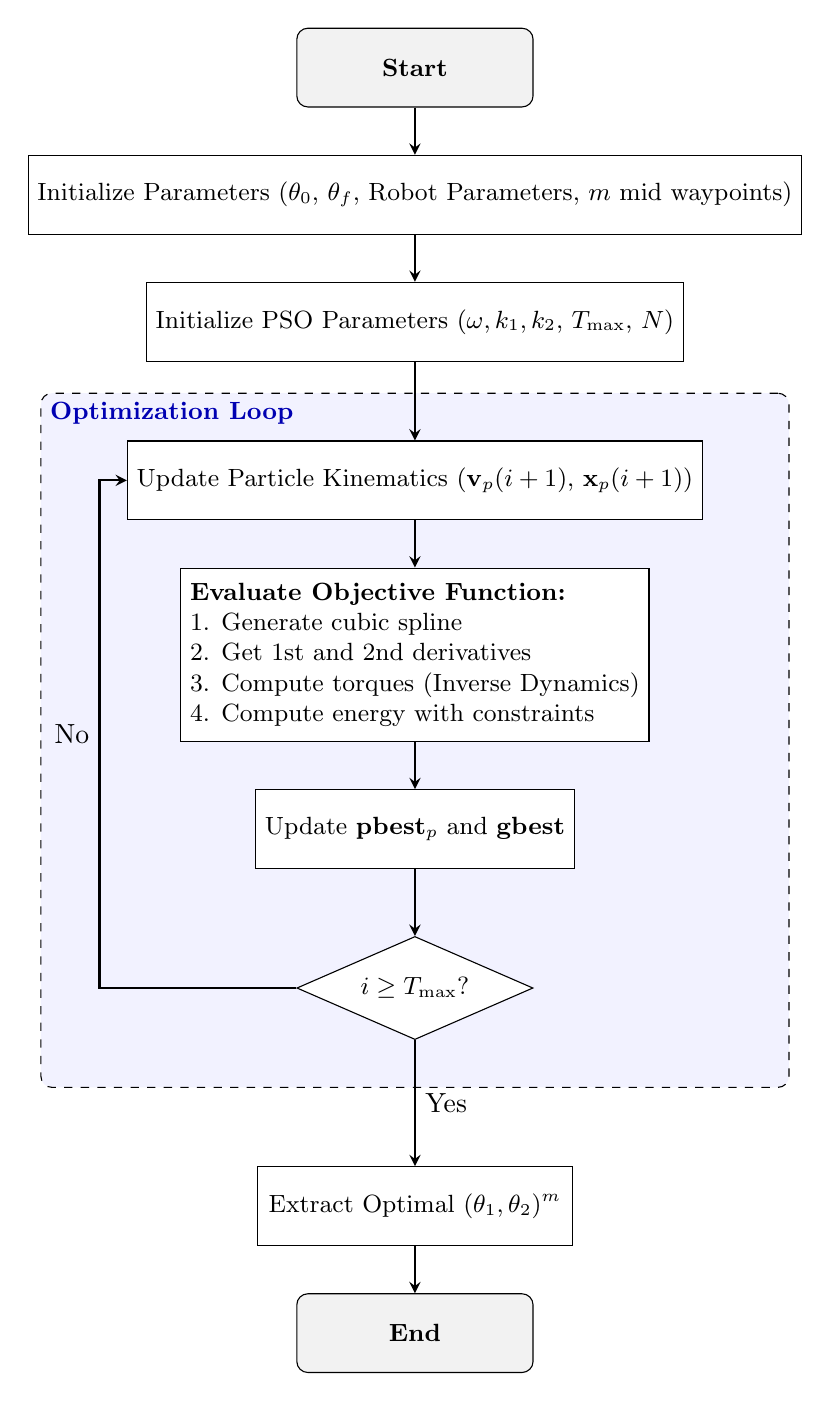
\begin{tikzpicture}[node distance=0.6cm, auto]

    % --- Estilos ---
    \tikzset{
        startstop/.style={rectangle, rounded corners, minimum width=3cm, minimum height=1cm,text centered, draw=black, fill=gray!10, font=\small\bfseries},
        process/.style={rectangle, minimum width=4cm, minimum height=1cm, text centered, draw=black, fill=white, font=\small},
        detailprocess/.style={rectangle, minimum width=5cm, minimum height=2.2cm, draw=black, fill=white, font=\small, align=left},
        decision/.style={diamond, aspect=2, minimum width=3cm, minimum height=1cm, text centered, draw=black, fill=white, font=\small},
        arrow/.style={thick,->,>=stealth},
        container/.style={draw, rectangle, minimum width = 9.5cm, minimum height=6.5cm, dashed, inner sep=0.6cm, rounded corners, fill=blue!5}
    }

    % --- Nodos ---
    \node (start) [startstop] {Start};
    \node (init) [process, below=of start] {Initialize Parameters ($\theta_0$, $\theta_f$, Robot Parameters, $m$ mid waypoints)};
    \node (pso) [process, below=of init] {Initialize PSO Parameters ($\omega, k_1, k_2$, $T_{\max}$, $N$)};
    
    % --- Optimization Loop Start ---
    \node (updkin) [process, below=of pso, yshift=-0.4cm] {
        Update Particle Kinematics  (\textbf{v}$_p(i+1)$, \textbf{x}$_p(i+1)$)
    };
    
    \node (eval) [detailprocess, below=of updkin] {
        \textbf{Evaluate Objective Function:} \\
        1. Generate cubic spline \\
        2. Get 1st and 2nd derivatives \\
        3. Compute torques (Inverse Dynamics) \\
        4. Compute energy with constraints
    };

    \node (update) [process, below=of eval] {Update \textbf{pbest}$_p$ and \textbf{gbest}};
    \node (dec1) [decision, below=of update, yshift=-0.25cm] {$i \geq T_{\max}$?};
    % --- Optimization Loop End ---
    
    \node (best) [process, below=of dec1, yshift=-1cm] {Extract Optimal $(\theta_{1},\theta_{2})^m$};
    \node (stop) [startstop, below=of best] {End};

    % --- Conexiones ---
    \draw [arrow] (start) -- (init);
    \draw [arrow] (init) -- (pso);
    \draw [arrow] (pso) -- (updkin);
    \draw [arrow] (updkin) -- (eval);
    \draw [arrow] (eval) -- (update);
    \draw [arrow] (update) -- (dec1);
    
    % Flecha del bucle de retorno al inicio del loop (Update Kinematics)
    \draw [arrow] (dec1.west) -- ++(-2.5,0) |- node [pos=0.25, left] {No} (updkin.west);
    
    \draw [arrow] (dec1) -- node [anchor=west] {Yes} (best);
    \draw [arrow] (best) -- (stop);

    % --- Recuadro del Bucle ---
    \begin{scope}[on background layer]
        \node[container, fit=(updkin) (eval) (update) (dec1)] (box) {};
        \node[blue!70!black, font=\small\bfseries, anchor=north west] at (box.north west) {Optimization Loop};
    \end{scope}

\end{tikzpicture}
    \caption{Flowchart of the proposed energy-efficient trajectory optimization using PSO and Quadratic Loss penalty functions.}
    \label{fig:pso_flowchart}
\end{figure}

\section{Results}
This section presents a simulation comparison between the proposed PSO-optimized trajectory and an arbitrary trajectory for the 2-DOF manipulator. The simulation was carried out using the robot and PSO algorithm parameters listed in table \ref{tab:params}.

\begin{table}[h]
\centering
\caption{Simulation parameters.}
\label{tab:params}
\begin{tabular}{|c|c|c|c|}
\hline
\multicolumn{2}{|c|}{\textbf{Robot Parameters}} & \multicolumn{2}{c|}{\textbf{PSO Parameters}} \\
\hline
\textbf{Parameter} & \textbf{Value [Units]} & \textbf{Parameter} & \textbf{Value} \\
\hline
$l_1,\  l_2$            & (0.5, 0.5) [m]                   & $w$         & 0.6 \\
$m_1, \ m_2$            & (5.0, 5.0) [kg]                  & $k_1$       & 1.4 \\
$r_1, \ r_2$            & ($0.5l_1,\ 0.5l_2$) [m]          &  $k_2$       & 1.4  \\
$I_1,\ I_2$            & (0.02, 0.15) [kg$\cdot$m$^2$]    &  $N$         & 50  \\
$T$                      & 4.0 [s]                   &   $T_{\max}$ &  200 \\
$\Delta t$            & 0.01 [s]                    &           &       \\
$m$                   & 2 [-]                     &             &     \\
$\tau_{\max}$         & 30.0 [N$\cdot$m]         &             &     \\
$\dot{\theta}_{\max}$ & 2.0 [rad/s]              &             &     \\
$\theta_0$            & $(\pi/6,\ \pi/3)$ [rad]   &             &     \\
$\theta_f$            & $(\pi/3,\ -\pi/6)$ [rad]  &             &     \\
\hline
\end{tabular}
\end{table}

Figure \ref{fig:trayectorias} shows the arbitrary trajectory generated using the velocity trapezoidal profile described in the previous section, and the trajectory corresponding to the proposal of this work. In addition, figure \ref{fig:joint_traj} illustrates the comparison of joint trajectories for both robot joints to provide better insight in system movement in cartesian space. Although the trajectory generated by the proposal is slightly longer than the arbitrary one, it is convenient to understand the behavior of the system in terms of joint torques and accumulated mechanical energy in order to grasp the form of the trajectory.

\begin{figure}[htbp]
    \centering
    
\includegraphics[width=\linewidth]{figures/Trayectorias.pdf}
    \caption{Generated trajectories for a 2-DOF manipulator robot. (a) Trajectory computed by the proposed algorithm; (b) Arbitrary trajectory computed using the velocity trapezoidal profile.}
    \label{fig:trayectorias}
\end{figure}

\begin{figure}[htbp]
    \centering
    
\includegraphics[width=\linewidth]{figures/Posiciones.pdf}
    \caption{Joint trajectories comparison for a 2-DOF robot manipulator. (a) Joint 1 trajectories; (b) Joint 2 trajectories.}
    \label{fig:joint_traj}
\end{figure}

Figure \ref{fig:cum_energy} shows accumulated energy over time, while figure \ref{fig:joint_torques} describes the behavior of torques over time for both joints of the robot manipulator.

In the case of joint 1 torque, the arbitrary trajectory maintains relatively high values with smooth but persistent variations in the approximate range of 29–32 Nm. In contrast, the PSO trajectory exhibits a notable reduction in torque in the central region of the movement, reaching a minimum near 17 Nm before returning to similar final values. This behavior suggests that the PSO algorithm redistributed acceleration and intermediate joint configurations to avoid maintaining high stress throughout the entire movement. Although the peak torque does not decrease drastically at this joint, the average stress is reduced during a significant portion of the range, which directly contributes to the reduction in overall energy consumption.

On the other hand, a more pronounced behavior is observed in torques for joint 2. The PSO trajectory exhibits an initial phase with a more pronounced negative torque, followed by a gradual transition to positive values. This variation indicates a more active use of the system's dynamics, possibly leveraging gravitational or inertial effects to subsequently reduce the net effort required.

The direct effects of these torque profiles are reflected in the accumulated energy graph, which shows a clear difference in the temporal evolution between the two trajectories. The trajectory generated using PSO exhibits a significant reduction in total energy consumption compared to the arbitrary trajectory. This optimized energy shows a low increasing rate of energy consumption in the intermediate region of the movement (approximately between 2 and 3 seconds), and the final accumulated value is considerably lower. According to the reported values in simulation, the total energy consumed by the PSO trajectory was \textbf{3013.21 J}, while the arbitrary trajectory reached \textbf{4120.05 J}, representing a \textbf{26.86\% improvement}. This reduction confirms that the optimization algorithm successfully redistributed the dynamic effort throughout the time interval, decreasing the total mechanical work required by the actuators.

Likewise, the overall peak torque recorded was \textbf{31.50 N m} for the PSO trajectory compared to \textbf{32.37 N m} for the arbitrary trajectory, representing a \textbf{2.67\% improvement}. While the percentage reduction in peak torque is smaller compared to the energy reduction, this result is consistent with the problem formulation: the quadratic penalty included in the objective function does not completely eliminate peaks, but rather discourages excessive values while simultaneously balancing the minimum energy criterion. This explains why the optimization prioritized a considerable reduction in total energy, keeping peak torque within a slightly lower range without sacrificing dynamic viability.

Although this peak torque reduction is relatively modest, its impact should not be underestimated in the context of actuator longevity. As stated in section 3, peak torque values are directly associated with thermal stress ---as higher torque demands result in increased current draw and, consequently, elevated temperatures within the actuator---. Even small reductions in peak torque can mitigate the amplitude of thermal cycles, which are a primary driver of material fatigue and insulation degradation over time. Therefore, a 2.67\% decrease in peak torque can contribute to reducing thermal cycling severity, potentially slowing down wear mechanisms and extending the service life of the actuators.

\begin{figure}[htbp]
    \centering
    
\includegraphics[width=\textwidth]{figures/Energia acumulada.pdf}
    \caption{Accumulated energy comparison using square torque metric.}
    \label{fig:cum_energy}
\end{figure}

\begin{figure}[htbp]
    \centering
    
\includegraphics[width=\textwidth]{figures/Torques.pdf}
    \caption{Torques comparison throughout time for both joints of the 2-DOF robot manipulator. (a) Torques comparison for joint 1; (b) Torques comparison for joint 2.}
    \label{fig:joint_torques}
\end{figure}

Figure \ref{fig:vels} shows a comparison of joint velocities for both joints of the 2-DOF robot manipulator. The optimized joint velocity profiles reflect the influence of torque and velocity penalties included in the cost function. Compared to the arbitrary trajectory, the PSO solution redistributes motion over time, increasing velocity in dynamically favorable regions and reducing it where higher torques are required. Both joints exhibit smooth and bounded velocity profiles, ensured by the cubic spline parameterization and velocity constraints and contributing to lower energy consumption while maintaining kinematic feasibility.

To assess the influence of PSO parameter selection on the optimization outcome, a sensitivity analysis was performed by varying the inertia weight $w$ and the acceleration 
coefficients $k_1$ and $k_2$ around the baseline configuration. The results are summarized in Table~\ref{tab:sensitivity}. 

Across all tested configurations, the total energy consumed ranged from 3013.21~J to 3016.45~J, representing a variation of less than 0.11\% relative to the best result. This narrow spread indicates that the proposed method is largely insensitive to moderate changes in PSO parameters, and that the baseline configuration ($w = 0.6$, $k_1 = k_2 = 1.4$) consistently yields near-optimal performance. These findings suggest that the optimization landscape shaped by the proposed cost function is sufficiently well-conditioned to guide the swarm toward similar solutions regardless of the specific parameter combination.

\begin{table}[ht]
\centering
\caption{PSO sensitivity analysis: total energy consumed under 
         different parameter configurations.}
\label{tab:sensitivity}
\begin{tabular}{|c|c|c|c|}
\hline
\textbf{$w$} & \textbf{$k_1$} & \textbf{$k_2$} & 
\textbf{Energy [J]} \\
\hline
0.3 & 1.4 & 1.4 & 3016.45 \\
0.6 & 1.4 & 1.4 & \textbf{3013.21}\\
0.9 & 1.4 & 1.4 & 3015.96 \\
0.6 & 1.0 & 1.0 & 3015.25 \\
0.6 & 2.0 & 2.0 & 3015.25 \\
0.6 & 1.4 & 2.0 & 3014.78 \\
0.6 & 2.0 & 1.4 & 3015.95 \\
\hline
\end{tabular}
\end{table}

\begin{figure}[htbp]
    \centering
    
\includegraphics[width=\textwidth]{figures/Velocidades.pdf}
    \caption{Joint velocities comparison for the 2-DOF robot manipulator. (a) Joint velocities comparison for joint 1; (b) Joint velocities comparison for joint 2.}
    \label{fig:vels}
\end{figure}

\section{Conclusions}
This paper presented a proof-of-concept trajectory planning strategy for a 2-DOF manipulator robot aimed at minimizing energy consumption through the combination of cubic spline interpolation and PSO. The proposed method formulated trajectory generation as a constrained optimization problem in joint space, incorporating penalty terms on torque and joint velocity to ensure dynamically feasible and safe actuator operation.

Simulation results suggest that the optimized trajectory successfully redistributed the dynamic effort throughout the motion, producing smoother torque and velocity profiles 
while maintaining constraint compliance. Under the simulated scenario, the method achieved a reduction in total energy consumption of approximately 26.86\% compared to an arbitrary trajectory, together with a slight reduction in peak torque. These results indicate that optimizing intermediate joint configurations shows promise for improving energetic efficiency without modifying the robot hardware or execution time. While encouraging, these findings are based on a single simulated scenario and should not be generalized to broader industrial settings without further validation.

Although the optimization process involves the selection of PSO parameters, the sensitivity analysis conducted over a representative range of inertia weights and acceleration coefficients revealed that the method's performance is robust to parameter variation, showing a difference of less than 0.11\% in total energy consumption across all tested configurations.

Future work will focus on validating the approach experimentally on physical hardware, extending it to manipulators with higher degrees of freedom, incorporating real actuator models and exploring adaptive or hybrid optimization strategies to improve convergence speed and robustness. Such extensions are necessary to assess the scalability and practical applicability of the proposed method beyond the simulation environment.
 
%Multiple citations are grouped \cite{ref_article1,ref_lncs1,ref_book1}, \cite{ref_article1,ref_book1,ref_proc1,ref_url1}.

%
% ---- Bibliography ----
%
% BibTeX users should specify bibliography style 'splncs04'.
% References will then be sorted and formatted in the correct style.
%
% \bibliographystyle{splncs04}
% \bibliography{mybibliography}
%
\begin{thebibliography}{8}

\bibitem{ref_industry5.0}
Xu, X.; Lu, Y.; Vogel-Heuser, B.; Wang, L. Industry 4.0 and Industry 5.0—Inception, conception and perception, Journal of Manufacturing Systems, 530-535, (2021)

\bibitem{ref_ind5.0_capabilities}
Kans, M.; Campos, J.; Digital capabilities driving industry 4.0 and 5.0 transformation: Insights from an interview study in the maintenance domain, Journal of Open Innovation: Technology, Market, and Complexity (2024)

\bibitem{ref_wr2025}
Müller, C.: World Robotics 2025 – Industrial Robots, IFR Statistical
Department, VDMA Services GmbH, Frankfurt am Main, Germany (2025)

\bibitem{ref_iea}
World - IEA, \url{https://www.iea.org/world/electricity}, Last accessed 3 Mar 2026

\bibitem{ref_eia}
U.S Energy Information Administration, \url{https://www.eia.gov/todayinenergy/detail.php?id=65264}, Last accessed 3 Mar 2026

\bibitem{ref_ceic}
CEIC, \url{https://www.ceicdata.com/en/china/electricity-consumption-by-industry/cn-electricity-consumption-industry}, Las accessed 3 Mar 2026

\bibitem{soori2023}
Soori, M., Arezoo, B., Dastres, R.: Optimization of Energy 
Consumption in Industrial Robots, A Review. Cognitive Robotics 3, 142--157 (2023).

\bibitem{zhou2024}
Zhou, Y., Han, G., Wei, Z., Huang, Z., Chen, X., Wu, J.: Optimal Trajectory Planning of Robot Energy Consumption Based on Improved Sparrow Search Algorithm. Measurement and Control (2024).

\bibitem{zhang2023}
Zhang, S., et al.: Multi-Objective Optimal Trajectory Planning for Robotic Arms Using Deep Reinforcement Learning. Sensors 23(13), 5974 (2023).

\bibitem{garriz2022}
Garriz, C., Domingo, R.: Trajectory Optimization in Terms of Energy and Performance of an Industrial Robot in the Manufacturing Industry. Sensors 22(19), 7538 (2022). 

\bibitem{ref_dynamics1}
Dona’, D.; Bettega, J.; Tamellin, I.; Boscariol, P.; Caracciolo, R. Minimum-Energy Trajectory Planning for an Underactuated Serial Planar Manipulator. Robotics 2025, 14, 98

\bibitem{ref_dynamics2}
Vishnu Varthan, R.; Sanjay Ganesh, S.; Anbarasi M. P.: Energy-Efficient Trajectory Tracking of a 2-DOF Planar Manipulator Using Optimized Computed Torque Control. IJRASET (2026)

\bibitem{ref_polyint}
Siciliano, B.; Sciavicco, L.; Villani, L.; Oriolo, G.: Robotics: Modelling, Planning and Control. Springer Science \& Business Media, UK (2010)

\bibitem{ref_pso}
Kennedy, J.; Ebenhart, R.: Particle swarm optimization. IEEE Xplore, 1944-1947 (1995)

\bibitem{ref_pso_adv}
Angeline, P.: Evolutionary optimization versus particle swarm optimization: Philosophy and performance differences. Evolutionary Programming VII (pp. 601-610). Springer (1998)

\bibitem{ref_peakcurrent}
Ehsani M., Gao Y., Longo, S.; Ebrahimi, K. : Modern Electric, Hybrid Electric, and Fuel Cell Vehicles, 3rd ed. Boca Raton, USA, 2019, pp. 325-360

\bibitem{ref_penaltyfunc}
J. Nocedal and S. J. Wright, Numerical Optimization, 2nd ed. New York, NY, USA: Springer, 2006

\bibitem{ref_quadloss}
M. S. Bazaraa, H. D. Sherali, and C. M. Shetty, Nonlinear Programming: Theory and Algorithms, 3rd ed. Hoboken, NJ, USA: Wiley-Interscience, 2006.

\bibitem{ref_csape}
Mathworks - csape, \url{https://la.mathworks.com/help/curvefit/csape.html}, Last accessed 4 Mar 2026

\bibitem{ref_trap_traj}
MathWorks - Trajectory Planning for Robot Manipulators, \url{https://blogs.mathworks.com/student-lounge/2019/11/06/robot-manipulator-trajectory/} last accessed 9 Apr 2026

%journal articles -> Author, F.: Article title. Journal \textbf{2}(5), 99--110 (2016)
% LNCS Chapters -> Author, F., Author, S.: Title of a proceedings paper. In: Editor, F., Editor, S. (eds.) CONFERENCE 2016, LNCS, vol. 9999, pp. 1--13. Springer, Heidelberg (2016). \doi{10.10007/1234567890}
% Book -> Author, F., Author, S., Author, T.: Book title. 2nd edn. Publisher, Location (1999)
% Proceedings wo editors -> Author, A.-B.: Contribution title. In: 9th International Proceedings on Proceedings, pp. 1--2. Publisher, Location (2010)
% Homepage -> LNCS Homepage, \url{http://www.springer.com/lncs}. Last accessed 4 Oct 2017
\end{thebibliography}
\end{document}